\section{Architecture Design Patterns}

\subsection{Decision for Dotnet framework}
\label{ssec:dotnet}

MVC\footnote{MVC: Model View Controller} is one of the many architectural patterns, which provide a common reusable solution in a software system.
This is presumably by far the most used designed pattern adapted by many frameworks like
Microsoft .NET core MVC, 
Java Spring framework MVC etc. 

\begin{figure}[H]
    \centering 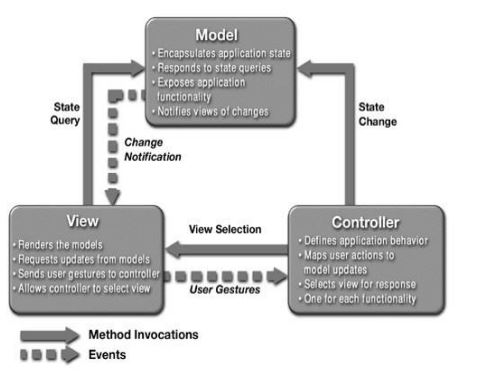
\includegraphics{grafiken/mvc_hotop.jpg}
    \caption{MVC Overview \cite{Hotop2015}}
    \label{fig:mvcOverview}
\end{figure}

\par
   The main idea behind is to make a clear separation between domain object and the presentation layer. The two elements should be completely self-
   contained and should be able to work without the presence of the other. This 
   architecture acknowledges three primary aspects. Figure \ref{fig:mvcOverview} 
   gives us an overview of MVC pattern.
   \begin{enumerate}
       \item 
        \textbf{The Model}: This is the layer which represents the data layer. It 
        contains all the relevant data for the business logic.

       \item 
        \textbf{The View}: This is the user interface where the graphical units area
        placed like buttons, text etc.

       \item 
        \textbf{The Controller} : This layer takes the inputs and changes the two other
        layer accordingly.
   \end{enumerate} 